%# -*- coding: utf-8 -*-
% tiling.tex
% asymptotebyexample 的一章,曲线绘制和编程入门

\chapter{André Deledicq 的铺砌插画}
\label{chap:tiling}

André 是一名兴趣广泛的法国数学教师,在他的新著《Le monde des pavages》(《铺
砌世界》)中,打算画一幅有关羊的铺砌插画:
\begin{figure}[H]
  \centering
  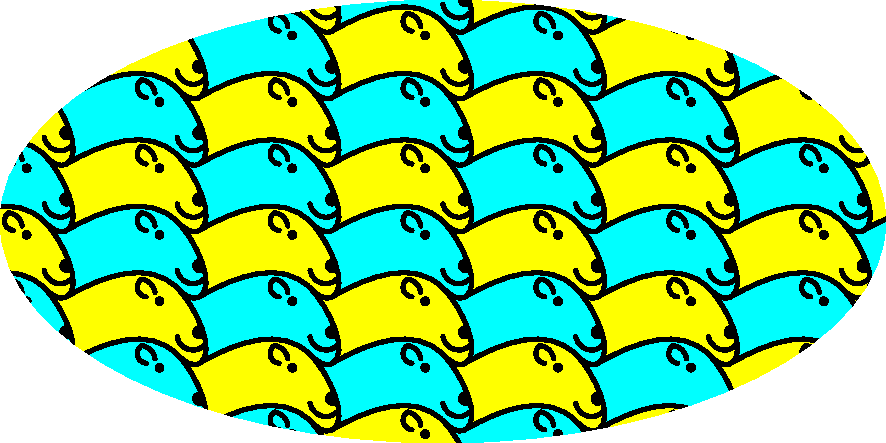
\includegraphics{tiling.pdf}
  \caption{André 理想中的铺砌图}
  \label{fig:tiling}
\end{figure}

André 很清楚他要画的图形的数学理论,但 André 的朋友 Timothy 告诉他要画这样
的图形多少是需要一些编程的知识的,对于他这样一位往日对计算机并不通晓的人来说
可能会有困难。不过 André 并不以为意:这世上还有什么比数学更难的呢?于是他兴
致勃勃的开始了。

\section{从矩形到铺砌}
\label{sec:rect2tiling}

铺砌图,顾名思义,就是像铺地板砖一样,把许多相同样式的图形平铺开来。不过,并
不是什么图形都可以平铺填满整个平面的——比如圆形就不行。把许多圆形一个挨一个
排列起来,也只能得到
\begin{figure}[H]
\centering
\begin{asy}
size(0,2cm);
for (int i = 0; i < 3; ++i)
    for (int j = 0; j < 10; ++j)
        filldraw(circle((j,i), 0.5), lightblue);
\end{asy}
\end{figure}
\noindent 或者是
\begin{figure}[H]
\centering
\begin{asy}
size(0,2cm);
for (int i = 0; i < 3; ++i)
    for (int j = 0; j < 10; ++j)
        filldraw(circle((j+0.5(i%2),sqrt(3)/2*i), 0.5), lightblue);
\end{asy}
\end{figure}
\noindent 都会留下许多空隙。而矩形、平行四边形、六边形等等都可以不留空隙地把平面铺满。

但问题是,如何设计出 André 理想中的那种看起来形状不规则的铺砌图案呢?

身为数学教师的 André 当然有办法。其实不规则铺砌图案还是规则图案的变形。
André 要画的羊形铺砌图,其实就是从矩形铺砌变化而来的。只要把一个矩形图案的上
下两边、左右两边分别变形,使得变形后的上边与下边、左边与右边还对应重合,就依
然可以完美地拼合起来。这正是铺砌图案最基本的构成方式:
\begin{figure}[H]
\centering
\begin{asy}
size(0,5cm);
defaultpen(linewidth(1mm));
guide rec = box((0,0), (2,1));
draw(rec);

draw(shift(3,0)*rec, gray+0.5mm);
guide left = (0,1) -- (-0.2,0.8) -- (0,0.6) -- (0.1,0.1) -- (0,0);
guide bot = (0,0) -- (0.2,0.1) -- (1.6,-0.1) -- (2,0);
draw(shift(3,0) * (left ^^ shift(2,0)*left), heavyblue);
draw(shift(3,0) * (bot ^^ shift(0,1)*bot), heavygreen);

guide shape = left & bot & shift(2,0)*reverse(left)
    & shift(0,1)*reverse(bot) & cycle;
for (int i = 0 ; i < 2; ++i)
    for (int j = 0; j < 4; ++j)
	filldraw(shift(0.5+j,-1.5+0.5i)*scale(0.5)*shape, lightblue);
\end{asy}
\end{figure}

有了这个方法,对复杂的铺砌图,也只要从一个基本形状(比如矩形、正六边形)开始
变形,就等到铺砌所需要的一块“砖”。

因此,要画出羊头形状铺砌图,只要把一个矩形按照上面的要求变形为一个羊头形状,
在不同的位置重复画出就可以了。

\section{变量与曲线}

下面的问题就是,怎么画一个羊头呢?更具体地说,怎么画出羊头的曲线呢?

那么,首先要了解如何在 \Asy{} 中描述曲线。\ref{sec:linedraw} 节中提到 |--| 连
结一组坐标就成为直(折)线段;类似地,用 |..|\index{..@\asyinline=..=} 连结坐
标就得到经过这些坐标点的曲线:
\begin{asycode}
size(5cm,0);
pair z1 = (0,1), z2 = (1,1), z3 = (2,1),
     z4 = (0,0), z5 = (1,0), z6 = (2,0);
guide p = z4 .. z1 .. z2 .. z6;
draw(p, gray+2mm);
\end{asycode}
\begin{figure}[H]
  \centering
\begin{asy}
size(5cm,0);
pair z1 = (0,1), z2 = (1,1), z3 = (2,1),
     z4 = (0,0), z5 = (1,0), z6 = (2,0);
guide p = z4 .. z1 .. z2 .. z6;
draw(p, gray+2mm);
dot(Label("1", align=NW), z1);
dot(Label("2", align=NE), z2);
dot("3", z3);
dot("4", z4);
dot("5", z5);
dot("6", z6);
\end{asy}
\end{figure}

在这里,我们定义了一些变量\index{变量}以使代码清晰(这里略去了画点和标签的代
码)。|pair|\index{pair@\asyinline=pair=} 类型的变量 |z1|, \ldots, |z6| 保存
六个坐标\index{坐标},|guide|\index{guide@\asyinline=guide=} 类型的变量 |p| 
保存一条曲线的路向\index{路向}。因而上面 |size| 之后的绘图代码就相当于
\begin{asycode}
draw( (0,0) .. (0,1) .. (1,1) .. (2,0), gray+2mm );
\end{asycode}
其中前面的一句 |size(5cm,0)|\index{size@\asyinline=size=} 表示代码中的坐标只
是相对位置,最后将整个图形按比例放缩为 $5$\,cm 宽\footnote{注意坐标、图形会被
放缩,但画笔的宽度不会放缩。}。类似地,也可以使用 |size(0,4cm)| 把图形放缩到
$4$\,cm 高。

最重要的当然还是曲线的表示。以 |..| 连结的坐标会以一种尽量接近圆弧的方式连为
经过这些点的光滑曲线。与画直线类似,|cycle|\index{cycle@\asyinline=cycle=} 可
以作为一个特殊的坐标产生闭合曲线,即一条闭路向\index{路向!闭路向}:
\begin{asycode}
guide q = z4 .. z1 .. z2 .. z6 .. cycle;
draw(q, gray+2mm);
\end{asycode}
\begin{figure}[H]
  \centering
\begin{asy}
size(5cm,0);
pair z1 = (0,1), z2 = (1,1), z3 = (2,1),
     z4 = (0,0), z5 = (1,0), z6 = (2,0);
guide q = z4 .. z1 .. z2 .. z6 .. cycle;
draw(q, gray+2mm);
dot(Label("1", align=NW), z1);
dot(Label("2", align=NE), z2);
dot("3", z3);
dot("4", z4);
dot("5", z5);
dot("6", z6);
\end{asy}
\end{figure}

变量不仅仅是给了坐标、路向等对象一个简洁的名字,它也使得对同一个对象重复使用
并进行不同的操作变得十分方便:
\begin{asycode}
fill(q, lightblue);
draw(q, gray+2mm);
\end{asycode}
\begin{figure}[H]
  \centering
\begin{asy}
size(5cm,0);
pair z1 = (0,1), z2 = (1,1), z3 = (2,1),
     z4 = (0,0), z5 = (1,0), z6 = (2,0);
guide q = z4 .. z1 .. z2 .. z6 .. cycle;
fill(q, lightblue);
draw(q, gray+2mm);
dot(Label("1", align=NW), z1);
dot(Label("2", align=NE), z2);
dot("3", z3);
dot("4", z4);
dot("5", z5);
dot("6", z6);
\end{asy}
\end{figure}

就像使用 |box| 可以直接得到矩形一样,最常用的曲线:圆、椭圆和圆弧,也可以使用
现成的命令得到:
\begin{table}[H]
\noindent
\begin{tabular}{ll}
|circle(c, r)| & 圆心 |c|,半径 |r| 的圆,这是逆时针方向的闭曲线; \\
|ellipse(c, a, b)| & 中心为 |c|,长半轴 |a|,短半轴 |b| 的椭圆,这也是逆时针
方向的闭曲线; \\
|arc(c, r, angle1, angle2)| & 圆心 |c|,半径 |r|,角度从 |angle1| 到 |angle2|
的圆弧。
\end{tabular}
\end{table}

例如:
\begin{asycode}
filldraw( circle((0,0), 1cm), lightblue, gray+2mm );
draw( arc((5cm,0), 1cm, 45, 135), gray+2mm );
\end{asycode}
\begin{figure}[H]
\centering
\begin{asy}
filldraw( circle((0,0), 1cm), lightblue, gray+2mm );
draw( arc((5cm,0), 1cm, 45, 135), gray+2mm );
\end{asy}
\end{figure}

一条用 |cycle| 产生的闭路向和简单地把首尾结点重合的路向是非常不同的。首先,只
有闭路向可以填充颜色;其次,使用 |cycle| 连结的曲线在起点处是光滑连接的,而如
果只是首尾结点重合则不会光滑连接。试将下面的曲线 |q2| 与上面的曲线 |q| 比较:
\begin{asycode}
guide q2 = z4 .. z1 .. z2 .. z6 .. z4;
draw(q2, gray+2mm);
\end{asycode}
\begin{figure}[H]
\centering
\begin{asy}
size(5cm,0);
pair z1 = (0,1), z2 = (1,1), z3 = (2,1),
     z4 = (0,0), z5 = (1,0), z6 = (2,0);
guide q2 = z4 .. z1 .. z2 .. z6 .. z4;
draw(q2, gray+2mm);
dot(Label("1", align=NW), z1);
dot(Label("2", align=NE), z2);
dot("3", z3);
dot("4", z4);
dot("5", z5);
dot("6", z6);
\end{asy}
\end{figure}

现在有了绘制曲线的方法,画出一个羊头就只是把草稿上的坐标连接起来而已。André
有一个纸上的草图,于是在描出几个点以后,他很快得到这样的结果(这里给图形增加
了辅助网格):
\begin{asycode}
size(0,4cm);
pen outline = black+1mm;
// `\color{comment}头`
guide head = (0.5,-0.2) .. (0.6,0.5) .. (0.2,1.3) .. (0,1.5) .. (0,1.5)
    .. (0.4,1.3) .. (0.8,1.5) .. (2.2,1.9) .. (3,1.5) .. (3.2,1.3)
    .. (3.6,0.5) .. (3.4,-0.3) .. (3,0) .. (2.2,0.4) .. (0.5,-0.2) .. cycle;
filldraw(head, cyan, outline);
dot(head, red+1mm); // `\color{comment}画出羊头曲线上的结点`
// `\color{comment}五官`
fill( circle((2.65,1.25), 0.12), outline );
fill( (3.5,0.3) .. (3.35,0.45) .. (3.5,0.6) .. (3.6,0.4) .. cycle, outline );
draw( (3,0.35) .. (3.3,0.1) .. (3.6,0.05), outline );
draw( (2.3,1.3) .. (2.1, 1.5) .. (2.15,1.7), outline );
draw( (2.1,1.7) .. (2.35,1.6) .. (2.45,1.4), outline );
\end{asycode}
\begin{figure}[H]
  \centering
\begin{asy}
size(0,4cm);
import math;
add(scale(1/2)*shift(0,-1)*grid(8,5,gray));
dot(Label("$O$",align=left), 0);
label("$1$", (0,1), align=W); label("$2$", (0,2), align=W);
label("$1$", (1,-0.5), align=S); label("$2$", (2,-0.5), align=S);
label("$3$", (3,-0.5), align=S); label("$4$", (4,-0.5), align=S);
pen outline = black+1mm;
guide head = (0.5,-0.2) .. (0.6,0.5) .. (0.2,1.3) .. (0,1.5) .. (0,1.5)
    .. (0.4,1.3) .. (0.8,1.5) .. (2.2,1.9) .. (3,1.5) .. (3.2,1.3)
    .. (3.6,0.5) .. (3.4,-0.3) .. (3,0) .. (2.2,0.4) .. (0.5,-0.2) .. cycle;
filldraw(head, cyan, outline);
dot(head, red+1mm);
fill( circle((2.65,1.25), 0.12), outline );
fill( (3.5,0.3) .. (3.35,0.45) .. (3.5,0.6) .. (3.6,0.4) .. cycle, outline );
draw( (3,0.35) .. (3.3,0.1) .. (3.6,0.05), outline );
draw( (2.3,1.3) .. (2.1, 1.5) .. (2.15,1.7), outline );
draw( (2.1,1.7) .. (2.35,1.6) .. (2.45,1.4), outline );
\end{asy}
\end{figure}

在一开始,André 使用
\begin{asycode}
pen outline = black+1mm;
\end{asycode}
定义一个 |pen|\index{pen@\asyinline=pen=} 类型的变量 |outline| 表示用来画羊头
轮廓的画笔\index{画笔},以备使用。

然后,André 直接用 |..| 连结一组坐标来定义羊的头部轮廓:
\begin{asycode}
guide head = (0.5,-0.2) .. (0.6,0.5) .. (0.2,1.3) .. (0,1.5) .. (0,1.5)
    .. (0.4,1.3) .. (0.8,1.5) .. (2.2,1.9) .. (3,1.5) .. (3.2,1.3)
    .. (3.6,0.5) .. (3.4,-0.3) .. (3,0) .. (2.2,0.4) .. (0.5,-0.2) .. cycle;
\end{asycode}
需要尖角的时候,就使用重复的相同点(如这里的起点);曲线变化大的地方,取的点
也比较密集。

最后五官的绘制。眼睛是填充的小黑圆,鼻子是黑色的卵形,耳朵和嘴都是简单的曲线。

于是,只要把这样一个图形一个挨一个地重复画许多遍,就可以得到 André 想要的铺
砌效果了。设计羊头形状的工作无疑是最关键也最复杂的,因此 André 的任务现在就
已经完成了一半。

不过继承了法国完美主义风气的 Deledicq 老师,很快挑出了毛病:这只羊头部的轮廓,
并不完全是按照 \ref{sec:rect2tiling} 节对矩形变形得到的——他的手稿基本上是这
样设计的,但在使用 \Asy{} 上绘图时则只是在手稿上相当随意地取了一些结点连结得
到曲线,这个轮廓想必也并不能严丝合缝地一个个拼起来。还有一件很令他恼火的事情
则是:要画出羊头的轮廓,他要画的点太多了,一个尖角用两个结点表示,也太不符合
他的简洁美学了。因此,这个看上去相当不错的羊头一号,就被 Deledicq 老师无情地否
决掉了。他决定发扬数学教师严谨简洁的作风,再做出更完美的羊头二号来。

\section{细致的曲线调整与曲线操作}
\label{sec:curve}

在 \Asy{} 中,除了简单地使用 |--| 和 |..| 连接坐标来定义直线与曲线以外,也提
供了更丰富的手段来对曲线进行更为细致的调整与操作。于是,就有了方向、张力、卷
曲值这些东西。

在曲线的结点处,可以使用以花括号括起的一个向量坐标来限定曲线在此处的切线方向
\index{方向}。例如:
\begin{asycode}
draw(z4 .. z2 .. z6, gray+2mm);
draw(z4{right} .. z2{right} .. z6{right}, heavyblue+2mm);
\end{asycode}
\begin{figure}[H]
  \centering
\begin{asy}
size(5cm,0);
pair z1 = (0,1), z2 = (1,1), z3 = (2,1),
     z4 = (0,0), z5 = (1,0), z6 = (2,0);
draw(z4 .. z2 .. z6, gray+2mm);
draw(z4{right} .. z2{right} .. z6{right}, heavyblue+2mm);
dot(Label("1", align=up), z1);
dot(Label("2", align=up), z2);
dot(Label("3", align=up), z3);
dot(Label("4", align=down), z4);
dot(Label("5", align=down), z5);
dot(Label("6", align=down), z6);
\end{asy}
\end{figure}
在这里,常量 |right| 就相当于罗盘方向 |E|,也就是 |(0,1)|。事实上,在 \Asy{}
中已经预定义好了上下左右四个方向:|up|\index{up@\asyinline=up=},
|down|\index{down@\asyinline=down=}, |left|\index{left@\asyinline=left=},
|right|\index{right@\asyinline=right=},作为四个罗盘方向的同义词。此外,也可
以使用预置的函数 \lstinline[language=Asymptote,mathescape]|dir($\text{角度}$)|
\index{dir@\asyinline=dir=} 来表示指向此方向的单位向量,例如:
\begin{asycode}
draw(z4 .. z2 .. z6, gray+2mm);
draw(z4{dir(60)} .. z2{dir(30)} .. z6{dir(-120)}, heavyblue+2mm);
\end{asycode}
\begin{figure}[H]
  \centering
\begin{asy}
size(5cm,0);
pair z1 = (0,1), z2 = (1,1), z3 = (2,1),
     z4 = (0,0), z5 = (1,0), z6 = (2,0);
draw(z4 .. z2 .. z6, gray+2mm);
draw(z4{dir(60)} .. z2{dir(30)} .. z6{dir(-120)}, heavyblue+2mm);
dot(Label("1", align=up), z1);
dot(Label("2", align=up), z2);
dot(Label("3", align=up), z3);
dot(Label("4", align=down), z4);
dot(Label("5", align=down), z5);
dot(Label("6", align=down), z6);
\end{asy}
\end{figure}
当然,这里并不要求使用单位向量来限定曲线方向,使用任何长度的向量都得得到相同
的效果。

就像上面的例子,限定曲线的切线方向无疑使得定义一条曲线更加直观和方便。不仅如
此,我们甚至还可以在曲线同一结点的两侧设置截然不同的切线方向,此时曲线就会在
这个结点的位置得到一个尖角。如:
\begin{asycode}
draw(z4 .. z2 .. z6, gray+2mm);
draw(z4 .. {up} z2 {down} .. z6, heavyblue+2mm);
\end{asycode}
\begin{figure}[H]
  \centering
\begin{asy}
size(5cm,0);
pair z1 = (0,1), z2 = (1,1), z3 = (2,1),
     z4 = (0,0), z5 = (1,0), z6 = (2,0);
draw(z4 .. z2 .. z6, gray+2mm);
draw(z4 .. {up} z2 {down} .. z6, heavyblue+2mm);
dot(Label("1", align=up), z1);
dot(Label("2", align=up), z2);
dot(Label("3", align=up), z3);
dot(Label("4", align=down), z4);
dot(Label("5", align=down), z5);
dot(Label("6", align=down), z6);
\end{asy}
\end{figure}

了解了曲线的方向,再来看曲线的张力\index{张力}。大体上讲,这是一个相对模糊的
概念,因为它并不像曲线切线方向那样具有明确的几何特征。如果把结点看做是钉子,
而把 \Asy{} 的曲线看做是用若干钉子固定起来的一根弹簧或是硬橡皮绳,或许有助于
理解所谓张力的概念。在不同的钉子之间,弹簧的张力越大,弹簧就越趋于直线的紧绷
状态;反之,张力小时,弹簧就会因为松驰而自动张成圆弧状。张力用
\lstinline[language=Asymptote,mathescape]|tension $\text{张力值}$|
\index{tension@\asyinline=tension=} 来设定,张力值是不小于 $0.75$ 的实数,默
认值 $1$ 使得曲线最接近圆弧形状。例如:
\begin{asycode}
draw(z4 {up} .. tension 0.75 .. {down} z6, heavyblue+2mm);
draw(z4 {up} .. tension 1 .. {down} z6, gray+2mm);
draw(z4 {up} .. tension 1.5 .. {down} z6, heavygreen+2mm);
\end{asycode}
\begin{figure}[H]
  \centering
\begin{asy}
size(5cm,0);
pair z1 = (0,1), z2 = (1,1), z3 = (2,1),
     z4 = (0,0), z5 = (1,0), z6 = (2,0);
draw(z4 {up} .. tension 0.75 .. {down} z6, heavyblue+2mm);
label("$tension=0.75$", z4 {up} .. tension 0.75 .. {down} z6, align=LeftSide);
draw(z4 {up} .. tension 1 .. {down} z6, gray+2mm);
draw(z4 {up} .. tension 1.5 .. {down} z6, heavygreen+2mm);
label("$tension=1.5$", z4 {up} .. tension 1.5 .. {down} z6, align=RightSide);
dot(Label("1", align=up), z1);
dot(Label("2", align=up), z2);
dot(Label("3", align=up), z3);
dot(Label("4", align=down), z4);
dot(Label("5", align=down), z5);
dot(Label("6", align=down), z6);
\end{asy}
\end{figure}
注意张力不仅影响两个结点之间的曲线形状,临近结点间的曲线形状也会受到影响。如:
\begin{asycode}
draw(z4 .. tension 0.75 .. z2 .. z6, heavyblue+2mm);
draw(z4 .. tension 1 .. z2 .. z6, gray+2mm);
draw(z4 .. tension 1.5 .. z2 .. z6, heavygreen+2mm);
\end{asycode}
\begin{figure}[H]
  \centering
\begin{asy}
size(5cm,0);
pair z1 = (0,1), z2 = (1,1), z3 = (2,1),
     z4 = (0,0), z5 = (1,0), z6 = (2,0);
draw(z4 .. tension 0.75 .. z2 .. z6, heavyblue+2mm);
draw(z4 .. tension 1 .. z2 .. z6, gray+2mm);
draw(z4 .. tension 1.5 .. z2 .. z6, heavygreen+2mm);
dot(Label("1", align=up), z1);
dot(Label("2", align=up), z2);
dot(Label("3", align=up), z3);
dot(Label("4", align=down), z4);
dot(Label("5", align=down), z5);
dot(Label("6", align=down), z6);
\end{asy}
\end{figure}

比弹簧或橡皮绳更强的是,\Asy{} 曲线在结点两边的张力事实上也可以使用
\lstinline[language=Asymptote,mathescape]|tension $\text{起}$ and $\text{末}$|
来分开设定:
\begin{asycode}
draw(z4 {up} .. tension 1 .. {down} z6, gray+2mm);
draw(z4 {up} .. tension 0.75 and 2 .. {down} z6, heavyblue+2mm);
\end{asycode}
\begin{figure}[H]
  \centering
\begin{asy}
size(5cm,0);
pair z1 = (0,1), z2 = (1,1), z3 = (2,1),
     z4 = (0,0), z5 = (1,0), z6 = (2,0);
draw(z4 {up} .. tension 1 .. {down} z6, gray+2mm);
draw(z4 {up} .. tension 0.75 and 2 .. {down} z6, heavyblue+2mm);
dot(Label("1", align=up), z1);
dot(Label("2", align=up), z2);
dot(Label("3", align=up), z3);
dot(Label("4", align=down), z4);
dot(Label("5", align=down), z5);
dot(Label("6", align=down), z6);
\end{asy}
\end{figure}

最后来看卷曲度。卷曲度影响曲线端点的弯曲程度,它的语法和设定曲线方向类似:
\lstinline[language=Asymptote,mathescape]|{curl $\text{数值}$}|\index{curl@\asyinline=curl=}。卷
曲度是一个非负值,其数值越大则曲线在端点的曲率越大,数值为 $0$ 时则曲率趋于
$0$。在曲线的端点处,有默认的卷曲度 $1$,使得曲线接近圆弧。例如:
\begin{asycode}
draw(z4 {curl 0} .. z0 .. {curl 0} z6, heavyblue+2mm);
draw(z4 {curl 1} .. z0 .. {curl 1} z6, gray+2mm);
draw(z4 {curl 5} .. z0 .. {curl 5} z6, heavygreen+2mm);
\end{asycode}
\begin{figure}[H]
  \centering
\begin{asy}
size(5cm,0);
pair z1 = (0,1), z2 = (1,1), z3 = (2,1),
     z4 = (0,0), z5 = (1,0), z6 = (2,0),
	 z0 = (1,2);
draw(z4 {curl 0} .. z0 .. {curl 0} z6, heavyblue+2mm);
draw(z4 {curl 1} .. z0 .. {curl 1} z6, gray+2mm);
draw(z4 {curl 5} .. z0 .. {curl 5} z6, heavygreen+2mm);
dot(Label("1", align=up), z1);
dot(Label("2", align=up), z2);
dot(Label("3", align=up), z3);
dot(Label("4", align=down), z4);
dot(Label("5", align=down), z5);
dot(Label("6", align=down), z6);
dot(Label("0", align=up), z0);
\end{asy}
\end{figure}
必须注意的是,卷曲度影响的是曲线的首尾端点的弯曲情况;而如果某个结点原本不是
曲线的端点,那么曲线就会在此处折成尖角——特别地,如果相临端点都设置了卷曲度
值,那么这两个结点之间就会是一段直线。例如:
\begin{asycode}
draw(z4 .. z1 .. z0{curl 0} .. z3 .. z6, heavyblue+1mm);
draw(z4 .. z1 .. z0{curl 1} .. z3 .. z6, gray+1mm);
draw(z4 .. z1 .. z0{curl 5} .. z3 .. z6, heavygreen+1mm);
\end{asycode}
\begin{figure}[H]
  \centering
\begin{asy}
size(5cm,0);
pair z1 = (0,1), z2 = (1,1), z3 = (2,1),
     z4 = (0,0), z5 = (1,0), z6 = (2,0),
     z0 = (1,2);
draw(z4 .. z1 .. z0{curl 0} .. z3 .. z6, heavyblue+1mm);
draw(z4 .. z1 .. z0{curl 1} .. z3 .. z6, gray+1mm);
draw(z4 .. z1 .. z0{curl 5} .. z3 .. z6, heavygreen+1mm);
dot(Label("1", align=up), z1);
dot(Label("2", align=up), z2);
dot(Label("3", align=up), z3);
dot(Label("4", align=down), z4);
dot(Label("5", align=down), z5);
dot(Label("6", align=down), z6);
dot(Label("0", align=up), z0);
\end{asy}
\end{figure}

除了直线连接的符号 |--| 和曲线连接的符号 |..|,还有几个连接点坐标以得到曲线的
连接符,它们分别是特殊的直线连接符 |---|\index{---@\asyinline=---=}、特殊的曲
线连接符 |::|\index{::@\asyinline=::=} 以及将曲线首尾相接的
|&|\index{&@\asyinline=&=}。再加上连接几条不同曲线的 |^^|,就是全部连接曲线的
符号了。

连接符 |---|\index{---@\asyinline=---=} 与 |--| 类似,都得到直线,单独使用
|---| 画出的直线和折线与使用 |--| 得到的结果并不能看出区别。但事实上,用
|---| 得到的并不是严格的直线折线,而只是非常接近直线的光滑曲线\footnote{在
\Asy{} 内部,连接符 \asyinline=---= 是
\asyinline=.. tension atleast infinity ..= 的缩写。\asyinline=atleast= 关键字
一般并不直接使用,故本文不作讨论,可参考 \cite{knuth1986}。}。因而,如果把
|---| 与 |..| 配合使用,就能使得到的直线与曲线光滑地连接,而不像使用 |--| 那
样得到不需要的尖角。例如:
\begin{asycode}
draw(z6 .. z4 -- z1 .. z3 .. cycle, gray+2mm);
draw(z6 .. z4 --- z1 .. z3 .. cycle, heavyblue+1mm);
\end{asycode}
\begin{figure}[H]
  \centering
\begin{asy}
size(5cm,0);
pair z1 = (0,1), z2 = (1,1), z3 = (2,1),
     z4 = (0,0), z5 = (1,0), z6 = (2,0);
draw(z6 .. z4 -- z1 .. z3 .. cycle, gray+2mm);
draw(z6 .. z4 --- z1 .. z3 .. cycle, heavyblue+1mm);
dot(Label("1", align=left), z1);
dot(Label("2", align=right), z2);
dot(Label("3", align=right), z3);
dot(Label("4", align=left), z4);
dot(Label("5", align=right), z5);
dot(Label("6", align=right), z6);
\end{asy}
\end{figure}

连接符 |::|\index{::@\asyinline=::=} 则与 |..| 类似,都得到曲线\footnote{在
\Asy{} 内部,连接符 \asyinline=::= 是 \asyinline=.. tension atleast 1 ..= 的
缩写。\Asy{} 的曲线功能和语法大多源自 \MP{},不过在 \MP{} 中与 \asyinline=::=
功能相同的连接符是 \asyinline=...=。}。不过连接符 |::| 有一个特性,就是它将尽可能使两个坐标之间的曲线没有拐
点(即尽可能避免两坐标间出现 S 形曲线,效果是在 |..| 的基础上自动增加张力的结
果)。例如:
\begin{asycode}
draw(z4{up} .. z2{dir(40)} .. z3, gray+2mm);
draw(z4{up} :: z2{dir(40)} .. z3, heavyblue+1mm);
\end{asycode}
\begin{figure}[H]
  \centering
\begin{asy}
size(5cm,0);
pair z1 = (0,1), z2 = (1,1), z3 = (2,1),
     z4 = (0,0), z5 = (1,0), z6 = (2,0);
draw(z4{up} .. z2{dir(40)} .. z3, gray+2mm);
draw(z4{up} :: z2{dir(40)} .. z3, heavyblue+1mm);
dot(Label("1", align=right), z1);
dot(Label("2", align=right), z2);
dot(Label("3", align=right), z3);
dot(Label("4", align=right), z4);
dot(Label("5", align=right), z5);
dot(Label("6", align=right), z6);
\end{asy}
\end{figure}

|&|\index{&@\asyinline=&=} 连接符用于把几段首尾点依次重合的曲线直接相连,而不
改变原来连接前曲线的形状。这事实上与使用重复点直接用 |..| 生成尖角的效果相同
,但在 \Asy{} 中,连接符 |&| 会在生成的曲线中去除第一条曲线的尾结点(它应该是
与第二条曲线的首结点重合的),因而不会出现像之前直接使用 |..| 生成的曲线那样
会有重复的结点。例如:
\begin{asycode}
draw(z1{right} .. {down} z5 & z5 {up} .. {right}z3, gray+2mm);
\end{asycode}
\begin{figure}[H]
  \centering
\begin{asy}
size(5cm,0);
pair z1 = (0,1), z2 = (1,1), z3 = (2,1),
     z4 = (0,0), z5 = (1,0), z6 = (2,0);
draw(z1{right} .. {down} z5 & z5 {up} .. {right}z3, gray+2mm);
dot(Label("1", align=up), z1);
dot(Label("2", align=up), z2);
dot(Label("3", align=up), z3);
dot(Label("4", align=down), z4);
dot(Label("5", align=down), z5);
dot(Label("6", align=down), z6);
\end{asy}
\end{figure}
另一方面,相比直接单独绘制几条不相关的曲线,使用 |&| 连接符的一个重要作用是可
以由此生成合适的闭曲线。例如:
\begin{asycode}
filldraw(z1 .. z2 .. z6 & z6 .. z5 .. z1 & cycle, lightblue, gray+2mm);
\end{asycode}
\begin{figure}[H]
  \centering
\begin{asy}
size(5cm,0);
pair z1 = (0,1), z2 = (1,1), z3 = (2,1),
     z4 = (0,0), z5 = (1,0), z6 = (2,0);
filldraw(z1 .. z2 .. z6 & z6 .. z5 .. z1 & cycle, lightblue, gray+2mm);
dot(Label("1", align=up), z1);
dot(Label("2", align=up), z2);
dot(Label("3", align=up), z3);
dot(Label("4", align=down), z4);
dot(Label("5", align=down), z5);
dot(Label("6", align=down), z6);
\end{asy}
\end{figure}

连接符 |^^|\index{^^@\asyinline=^^=} 在前面 \autoref{sec:linedraw} 中已经介绍
过了。这里则指出它的一个特殊应用:在一个区域中“挖洞”填充。在数学中,平面上
的一条简单闭曲线有的方向可以分为正负两种,逆时针方向为正,正时针方向为负。因
此,在某个方向曲线围成的区域中用连接符 |^^| 加入一条反方向的闭曲线,就相当于
在这个封闭区域中挖了一个洞。

在给出相关的例子之前,我们首先给出 \Asy{} 中把曲线方向逆转的函数
\lstinline[language=Asymptote,mathescape]|reverse($\text{曲线}$)|%
\index{reverse@\asyinline=reverse=},它接受一条曲线(可以是路径或路向)作为参
数,并返回此曲线的逆方向曲线。绘制时给曲线加上箭头可以明显看出其方向:
\begin{asycode}
draw(z1 .. z2 .. z6, gray+1mm, Arrow);
draw(reverse(z1 .. z2 .. z6), heavyblue+0.5mm, Arrow);
\end{asycode}
\begin{figure}[H]
  \centering
\begin{asy}
size(5cm,0);
pair z1 = (0,1), z2 = (1,1), z3 = (2,1),
     z4 = (0,0), z5 = (1,0), z6 = (2,0);
draw(z1 .. z2 .. z6, gray+1mm, Arrow);
draw(reverse(z1 .. z2 .. z6), heavyblue+0.5mm, Arrow);
dot(Label("1", align=up), z1);
dot(Label("2", align=up), z2);
dot(Label("3", align=up), z3);
dot(Label("4", align=down), z4);
dot(Label("5", align=down), z5);
dot(Label("6", align=down), z6);
\end{asy}
\end{figure}
于是,利用这种机制,在大圆内加上一个反方向的圆,把这两条曲线用 |^^| 连接,就
可以用来填充得到环形:
\begin{asycode}
size(5cm, 0);
filldraw(circle((0,0), 2) ^^ reverse(circle((0,0), 1)), lightblue, gray+2mm);
\end{asycode}
\begin{figure}[H]
  \centering
\begin{asy}
size(5cm, 0);
filldraw(circle((0,0), 2) ^^ reverse(circle((0,0), 1)), lightblue, gray+2mm);
\end{asy}
\end{figure}

需要说明的是,使用 |&| 连接两条曲线,得到的结果是一条连续的曲线;而使用 |^^|
连接两条曲线,得到的结果并不是一条曲线,而只是把两条曲线合并在一起的曲线数组
(数组在稍后的章节介绍)。因而它们在使用时是不同的。

上面介绍的内容,差不多就是 \Asy{} 中全部基本的曲线控制方式了。有了这些,
Deledicq 老师就可以按照 \autoref{sec:rect2tiling} 中的方式,精确地设计羊头的轮
廓了。他分别定义羊头左边和下面的两根线:
\begin{asycode}
guide headleft = (0,1.5){SE} .. tension 1.4 .. (0.5,-0.2){dir(-150)} ..
      {NW}(0,0);
guide headbottom = (0,0){SE} .. {dir(30)}(0.5,-0.2) ..{SE}(3,0);
\end{asycode}
\begin{figure}[H]
  \centering
\begin{asy}
size(5cm, 0);
guide headleft = (0,1.5){SE} .. tension 1.4 .. (0.5,-0.2){dir(-150)} ..
     {NW}(0,0);
guide headbottom = (0,0){SE} .. {dir(30)}(0.5,-0.2) ..{SE}(3,0);
draw("headleft", headleft, heavyblue+2mm);
draw("headbottom", headbottom, heavygreen+1mm);
\end{asy}
\end{figure}
这里的两条曲线虽然看起来定义比较复杂,但它们都只是由三个结点连接而成的,定义
更为直观,且在数学上更加简单。此外,明确限定了两条曲线在结点处的切线方向,可
以保证它们可以精确拼接。于是,通过平移变换、使用 |reverse| 函数逆向并使用连接
符 |&| 的拼接,就可以得到完整的羊头轮廓了:
\begin{asycode}
guide head = headleft & headbottom &
    shift(3,0)*reverse(headleft) & shift(0,1.5)*reverse(headbottom) & cycle;
\end{asycode}
\begin{figure}[H]
  \centering
\begin{asy}
size(5cm, 0);
guide headleft = (0,1.5){SE} .. tension 1.4 .. (0.5,-0.2){dir(-150)} ..
     {NW}(0,0);
guide headbottom = (0,0){SE} .. {dir(30)}(0.5,-0.2) ..{SE}(3,0);
guide head = headleft & headbottom &
    shift(3,0)*reverse(headleft) & shift(0,1.5)*reverse(headbottom) & cycle;
filldraw(head, lightblue, gray+2mm);
\end{asy}
\end{figure}

下面,羊的眼睛(|eye|)、耳朵(|ear|)、鼻子(|muzzle|)和嘴(|mouth|)就比较
容易得到了:
\begin{asycode}
guide eye = circle((2.6,1.2), 0.1);
guide ear = (2.3,1.3) .. (2.1,1.5) .. (2.2,1.7)
    & (2.2,1.7) .. (2.4,1.6) .. (2.5,1.4);
guide muzzle = circle((3.5,0.5), 0.15);
guide mouth = (3,0.4) .. (3.4,0.1) .. (3.6,0.2);
\end{asycode}

于是,André 就这样画出了一个完整的青色羊头:
\begin{asycode}
size(5cm, 0);
filldraw(head, cyan, linewidth(1mm));
fill(eye ^^ muzzle);
draw(ear ^^ mouth, linewidth(1mm));
\end{asycode}
\begin{figure}[H]
  \centering
\begin{asy}
size(5cm, 0);
guide headleft = (0,1.5){SE} .. tension 1.4 .. (0.5,-0.2){dir(-150)} ..
     {NW}(0,0);
guide headbottom = (0,0){SE} .. {dir(30)}(0.5,-0.2) ..{SE}(3,0);
guide head = headleft & headbottom &
    shift(3,0)*reverse(headleft) & shift(0,1.5)*reverse(headbottom) & cycle;
guide eye = circle((2.6,1.2), 0.1);
guide ear = (2.3,1.3) .. (2.1,1.5) .. (2.2,1.7)
    & (2.2,1.7) .. (2.4,1.6) .. (2.5,1.4);
guide muzzle = circle((3.5,0.5), 0.15);
guide mouth = (3,0.4) .. (3.4,0.1) .. (3.6,0.2);
filldraw(head, cyan, linewidth(1mm));
fill(eye ^^ muzzle);
draw(ear ^^ mouth, linewidth(1mm));
\end{asy}
\end{figure}

挑剔的 André 对这个羊头的曲线感到满意,因为作为一个铺砌图形,它绘制得完全精
确。一个羊头已经可以很好地画出来了,剩下的问题就是重复地把这个羊头铺满平面,
开始“铺砖”了。

\section{循环与条件判断}

要在平面上铺满相同的图形,就需要反复地在不同的位置进行绘制。\Asy{} 中可以使用
循环语句来完成这种重复的工作。

最常用的循环语句是 |for|\index{for@\asyinline=for=} 循环,其基本语法是:
\begin{asycode}
for (`初始化`; `执行条件`; `循环增量`)
    `循环语句体`
\end{asycode}
在一个循环语句中,\Asy{} 首先运行初始化语句,随后开始不断运行循环语句体,每次
运行语句体前检查执行条件以判断是否开始,而在运行语句体后运行循环增量的语句。
例如下面的语句会画出起始角度为 $0^\circ$, $30^\circ$, $60^\circ$, $90^\circ$ 
的四条曲线:
\begin{asycode}
for (real angle = 0; angle <= 90; angle += 30)
    draw( (0,0){dir(angle)} .. {right}(6cm,0), gray+1mm );
\end{asycode}
\begin{figure}[H]
  \centering
\begin{asy}
for (real angle = 0; angle <= 90; angle += 30)
    draw( (0,0){dir(angle)} .. {right}(6cm,0), gray+1mm );
\end{asy}
\end{figure}
在初始化部分定义了一个实数\index{实数}(|real|\index{real@\asyinline=real=})
类型的变量 |angle|,初始值为 $0$;进入循环的执行条件是角度变量 |angle| 不大于
直角;而在每次循环体画完曲线后,变量 |angle| 的值就增加 $30^\circ$。这里复合
赋值运算符 |+=|\index{+=@\asyinline/+=/} 表示在变量原有的基础上累加,
|var += x| 就等价于 |var = var + x|,类似地减法、乘除法、取余数和乘方也有
|-=|\index{-=@\asyinline/-=/}、|*=|\index{*=@\asyinline/*=/}、
|/=|\index{/=@\asyinline+/=+}、|%=|\index{%=@\asyinline/%=/}、
|^=|\index{^=@\asyinline/^=/} 这几种对应的赋值形式。对于整数\index{整数}
(|int|\index{int@\asyinline=int=})类型的变量,还可以使用 |++var| 和 |--var|
分别表示 |var += 1| 和 |var -= 1|。

如果循环体的语句不止一个,可以用花括号把这些语句括起来。如:
\begin{asycode}
for (int i = 0; i < 5; ++i) {
    filldraw(circle((2i*cm,0), 1cm), lightblue, gray+1mm);
    draw( (2i*cm,-1cm) -- (2i*cm,1cm), gray+1mm);
}
\end{asycode}
\begin{figure}[H]
  \centering
\begin{asy}
for (int i = 0; i < 5; ++i) {
    filldraw(circle((2i*cm,0), 1cm), lightblue, gray+1mm);
    draw( (2i*cm,-1cm) -- (2i*cm,1cm), gray+1mm);
}
\end{asy}
\end{figure}

平面铺砌图形需要在横向和纵向两个方向重复延伸,因而可以使用两层嵌套的循环语句
来完成这种图形:
\begin{asycode}
for (real x = 0; x < 8cm; x += 2cm)
    for (real y = 0; y < 4cm; y += 1cm)
        filldraw(ellipse((x,y), 1cm, 0.5cm), lightblue, gray+1mm);
\end{asycode}
\begin{figure}[H]
  \centering
\begin{asy}
for (real x = 0; x < 8cm; x += 2cm)
    for (real y = 0; y < 4cm; y += 1cm)
        filldraw(ellipse((x,y), 1cm, 0.5cm), lightblue, gray+1mm);
\end{asy}
\end{figure}

因此,有了前面的准备工作,André 就很容易通过一个双重循环来做出羊头的铺砌形状
来:
\begin{asycode}
// `\color{comment}……相关曲线的定义同前`
size(7cm, 0);
for (int x = 0; x < 4; ++x) {
    for (int y = 0; y < 4; ++y) {
        transform pos = shift(3x, 1.5y);
        filldraw( pos * head, cyan, linewidth(2bp));
        fill( pos * (eye ^^ muzzle) );
        draw( pos * (ear ^^ mouth), linewidth(2bp));
    }
}
\end{asycode}
\begin{figure}[H]
  \centering
\begin{asy}
size(7cm, 0);
guide headleft = (0,1.5){SE} .. tension 1.4 .. (0.5,-0.2){dir(-150)} ..
     {NW}(0,0);
guide headbottom = (0,0){SE} .. {dir(30)}(0.5,-0.2) ..{SE}(3,0);
guide head = headleft & headbottom &
    shift(3,0)*reverse(headleft) & shift(0,1.5)*reverse(headbottom) & cycle;
guide eye = circle((2.6,1.2), 0.1);
guide ear = (2.3,1.3) .. (2.1,1.5) .. (2.2,1.7)
    & (2.2,1.7) .. (2.4,1.6) .. (2.5,1.4);
guide muzzle = circle((3.5,0.5), 0.15);
guide mouth = (3,0.4) .. (3.4,0.1) .. (3.6,0.2);
for (int x = 0; x < 4; ++x) {
    for (int y = 0; y < 4; ++y) {
        transform pos = shift(3x, 1.5y);
        filldraw( pos * head, cyan, linewidth(2bp));
        fill( pos * (eye ^^ muzzle) );
        draw( pos * (ear ^^ mouth), linewidth(2bp));
    }
}
\end{asy}
\end{figure}
在这里,André 使用关于整数变量 |x| 和 |y| 的二重循环来控制整个铺砌图。在循环
体中使用了变换\index{变换}类型
|transform|\index{transform@\asyinline=transform=} 的变量 |pos| 来保存从原点
到每一块铺砌图形元的平移变换。在绘图时,给每条曲线都使用 |pos| 进行变换,就可
以在正确的位置绘图,而不用直接修改原来的曲线。

现在,André 几乎已经得到了和\autoref{fig:tiling} 相同的图形了。不过在
\autoref{fig:tiling} 中,羊头的颜色是随位置交错变化的。一个笨办法是分别用两组
循环来画出黄色和青色的羊头,但这会带来很多重复的代码。因此 André 决定在循环
体内做一点手脚:出于数学教师的敏感,他发现羊头颜色的规律可以由整数
|x|${}+{}$|y| 的奇偶性来判定,于是只要在循环体内增加一点判断……

\Asy{} 的条件判断\index{条件判断}语句正好可以完成这项工作。条件判断语句的基本
语法是:\index{if@\asyinline=if=}
\begin{asycode}
// `\color{comment}只有一个分支`
if (`条件`)
    `条件为真执行的语句块`
// `\color{comment}有 else 块,有两个分支`
if (`条件`)
    `条件为真执行的语句块`
else
    `条件为假执行的语句块`
\end{asycode}
其中,可以用花括号括起多行的语句块。因而,可以使用如下的语句来通过判断
|x|${}+{}$|y| 的奇偶性来决定画笔的颜色:
\begin{asycode}
pen color;
if ( (x+y) % 2 == 0 )   // `\color{comment}判断 x+y 是否为偶数`
    color = cyan;
else
    color = yellow;
\end{asycode}

把上面的控制颜色的判断语句用到前面的循环体中,就可以得到交错色彩的铺砌图了:
\begin{asycode}
// `\color{comment}……相关曲线的定义同前`
size(7cm, 0);
for (int x = 0; x < 4; ++x) {
    for (int y = 0; y < 4; ++y) {
        transform pos = shift(3x, 1.5y);
        pen color;
        if ( (x+y) % 2 == 0 )
            color = cyan;
        else
            color = yellow;
        filldraw( pos * head, color, linewidth(2bp));
        fill( pos * (eye ^^ muzzle) );
        draw( pos * (ear ^^ mouth), linewidth(2bp));
    }
}
\end{asycode}
\begin{figure}[H]
  \centering
\begin{asy}
size(7cm, 0);
guide headleft = (0,1.5){SE} .. tension 1.4 .. (0.5,-0.2){dir(-150)} ..
     {NW}(0,0);
guide headbottom = (0,0){SE} .. {dir(30)}(0.5,-0.2) ..{SE}(3,0);
guide head = headleft & headbottom &
    shift(3,0)*reverse(headleft) & shift(0,1.5)*reverse(headbottom) & cycle;
guide eye = circle((2.6,1.2), 0.1);
guide ear = (2.3,1.3) .. (2.1,1.5) .. (2.2,1.7)
    & (2.2,1.7) .. (2.4,1.6) .. (2.5,1.4);
guide muzzle = circle((3.5,0.5), 0.15);
guide mouth = (3,0.4) .. (3.4,0.1) .. (3.6,0.2);
for (int x = 0; x < 4; ++x) {
    for (int y = 0; y < 4; ++y) {
        transform pos = shift(3x, 1.5y);
        pen color;
        if ( (x+y) % 2 == 0 )
            color = cyan;
        else
            color = yellow;
        filldraw( pos * head, color, linewidth(2bp));
        fill( pos * (eye ^^ muzzle) );
        draw( pos * (ear ^^ mouth), linewidth(2bp));
    }
}
\end{asy}
\end{figure}

至此,André 大松一口气,他的铺砌图形基本上就绘制完成了。不过在他结束这一切的
时候,他的同事,\Asy{} 的专家 Philippe 告诉他,其实有关条件判断的语句还可以使
用一个条件表达式来简化。在这里,要判断的条件比较简单,而判断的结果也只是青、
黄两种颜色的值,因此,可以使用条件运算符\index{条件运算符}
|? :|\index{? :@\asyinline=? :=} 来代替。条件运算符是一个特殊的三元运算符
\index{三元运算符},它的语法是:
\begin{asycode}
`条件` ? `条件为真的值` : `条件为假的值`
\end{asycode}
因此前面的颜色判断和赋值语句就可以简化为:
\begin{asycode}
pen color = (i+j)%2==0 ? cyan : yellow;
\end{asycode}

现在,André 的铺砌图形就完成了。下面只要把他的图形剪裁一下,就大工告成了。


\section{图形的剪裁与自定义图}
\label{sec:clippicture}

André 最后的问题是把整个铺砌图形剪裁为椭圆形。为此,我们就需要引入在画线
(|draw|)、填充(|fill|)、标注(|label|)之外的最后一种基本绘图命令,即剪裁
(|clip|)\index{剪裁}\index{clip@\asyinline=clip=}。剪裁命令的基本语法是:
\begin{asycode}
clip(`图`, `曲线`);     // `\color{comment}图的默认值是当前图 currentpicture`
\end{asycode}
如果省略 |picture| 类型的图参数,则剪裁命令会把当前正在绘制的图用给定的曲线裁
剪开来;显示指定图参数则只剪裁给定的图中的内容。

裁剪默认的当前图只是在绘图的最后进行的少许修饰,而事实上,|clip| 命令更多地是
用在明确指定的图上,以完成一些用其他方法难以达成的效果。在第\ref{chap:xiantu}
章中已经看到了产生一个带网格的图的 |grid| 函数与使用图的 |add| 函数,下面,我
们首先说明如何自定义图并在其上绘图。

自定义一个图只要定义一个 |picture|\index{picture@\asyinline=picture=} 类型的
变量。新定义的图相当于一块单独的画布,而画线、填充、标注这些命令都可以在最前
面加上图的参数,表示在某一个图上进行绘图。例如:
\begin{asycode}
picture mypic;      //`\color{comment}自定义图`
draw(mypic, (0,0) -- (3cm,4cm) -- (5cm,0) -- cycle, gray+2mm);  //`\color{comment}画三角形`
fill(mypic, circle((4cm,3cm), 1cm), lightblue);                 //`\color{comment}画圆`
label(mypic, "trangle", (0,0));     //`\color{comment}标注`
label(mypic, "circle", (3cm,2cm));
\end{asycode}
不过这些内容都是画在自定义的图 |mypic| 上的,而只有在默认图 |currentpicture|
上的内容才会真正输出被我们看到。因此,就又需要使用
\autoref{sec:transformmodule} 中提到过的 |add| 命令把自定义图 |mypic| 中的内
容加到 |currentpicture| 之上:
\begin{asycode}
add(mypic);
\end{asycode}
\begin{figure}[H]
  \centering
\begin{asy}
picture mypic;
draw(mypic, (0,0) -- (3cm,4cm) -- (5cm,0) -- cycle, gray+2mm);
fill(mypic, circle((3cm,2cm), 1cm), lightblue);
label(mypic, "triangle", (1cm,0), N);
label(mypic, "circle", (3cm,2cm));
add(mypic);
\end{asy}
\end{figure}

\index{add@\asyinline=add=}
|add| 函数还可以有更多的参数,更一般的形式是\footnote{\asyinline=add= 函数有
很多变形,还带有更多次要的参数,详细的语法形式参看手册 \cite{asyman} 和
\prgname{plain\_picture.asy} 中的源代码。}:
\begin{asycode}
// `\color{comment}可以利用 size 函数自动缩放`
add(`目标图`=currentpicture, `源图`, above=true);
// `\color{comment}不能自动缩放`
add(`目标图`=currentpicture, `源图`, `位置坐标`, above=true);
\end{asycode}
|add| 函数的意义是:把源图的内容加到目标图的上方或下方,并使源图的原点重合于
目标图的位置坐标,其中目标图的默认值是当前图 |currentpicture|,|above| 的真假
值控制目标图是否在源图的上方,位置坐标不指定的形式两图原点重合。但需要注意,
带位置坐标的形式不支持利用 |size| 函数自动缩放,此时只能通过 |shift| 变换改变
源图的位置。通常,可以把目标图看做是已经有一些图案的背景画布,而源图是一些新
的图案,|add| 命令会把这些新的图案贴在原来画布的某个位置上。

使用自定义图的一个好处是,画在自定义图上的所有内容作为一个整体,可以通过
|add| 函数对其重复使用,或者进行各种操作(如仿射变换)。例如,对于前面定义的
图 |pic|,经过仿射变换\footnote{为方便文字标签的阅读,在 \Asy{} 中文字默认只
会旋转,不会倾斜。如果要求在图变换时,标签也随之变换产生特殊效果,可以修改
\asyinline=Label= 的 \asyinline=embed= 参数,参见 \cite{asyman}。}:
\begin{asycode}
add(mypic);
add(slant(1)*mypic, (5cm,0));
\end{asycode}
\begin{figure}[H]
  \centering
\begin{asy}
picture mypic;
draw(mypic, (0,0) -- (3cm,4cm) -- (5cm,0) -- cycle, gray+2mm);
fill(mypic, circle((3cm,2cm), 1cm), lightblue);
label(mypic, "triangle", (1cm,0), N);
label(mypic, "circle", (3cm,2cm));
add(mypic);
add(slant(1)*mypic, (5cm,0));
\end{asy}
\end{figure}

把剪裁命令用在自定义的图上,则这个图的内容就会随之被剪裁,在使用 |add| 时,即
可看到效果:
\begin{asycode}
add(mypic);                             // `\color{comment}增加未剪裁的图`
draw(circle((2cm,2cm), 2cm), red+1bp);  // `\color{comment}在未剪裁的图上画出剪裁圆形线`
clip(mypic, circle((2cm,2cm), 2cm));    // `\color{comment}用圆形剪裁`
add(mypic, (5cm,0));                    // `\color{comment}增加剪裁过的图`
\end{asycode}
\begin{figure}[H]
  \centering
\begin{asy}
picture mypic;
draw(mypic, (0,0) -- (3cm,4cm) -- (5cm,0) -- cycle, gray+2mm);
fill(mypic, circle((3cm,2cm), 1cm), lightblue);
label(mypic, "triangle", (1cm,0), N);
label(mypic, "circle", (3cm,2cm));
add(mypic);
draw(circle((2cm,2cm), 2cm), red+1bp);
clip(mypic, circle((2cm,2cm), 2cm));
add(mypic, (5cm,0));
\end{asy}
\end{figure}

剪裁命令的效果正是 André 需要的,为了用椭圆形剪裁图形,André 只需要对当前图
上的铺砌图进行剪裁。增加一句
\begin{asycode}
clip(ellipse((6,3), 5, 2));
\end{asycode}
就得到下图右侧的剪裁效果:
\begin{figure}[H]
  \centering
\begin{asy}
size(15cm, 0);
guide headleft = (0,1.5){SE} .. tension 1.4 .. (0.5,-0.2){dir(-150)} ..
     {NW}(0,0);
guide headbottom = (0,0){SE} .. {dir(30)}(0.5,-0.2) ..{SE}(3,0);
guide head = headleft & headbottom &
    shift(3,0)*reverse(headleft) & shift(0,1.5)*reverse(headbottom) & cycle;
guide eye = circle((2.6,1.2), 0.1);
guide ear = (2.3,1.3) .. (2.1,1.5) .. (2.2,1.7)
    & (2.2,1.7) .. (2.4,1.6) .. (2.5,1.4);
guide muzzle = circle((3.5,0.5), 0.15);
guide mouth = (3,0.4) .. (3.4,0.1) .. (3.6,0.2);
picture pic;
for (int x = 0; x < 4; ++x) {
    for (int y = 0; y < 4; ++y) {
        transform pos = shift(3x, 1.5y);
        pen color;
        if ( (x+y) % 2 == 0 )
            color = cyan;
        else
            color = yellow;
        filldraw(pic, pos * head, color, linewidth(2bp));
        fill(pic, pos * (eye ^^ muzzle) );
        draw(pic, pos * (ear ^^ mouth), linewidth(2bp));
    }
}
guide knife = ellipse((6,3), 5, 2);
draw(knife, red+2bp);
add(pic);
draw(knife, red+2bp);
draw(Label("clip", 3RightSide),
     (13,3) -- (15,3), squarecap+miterjoin+2mm, Arrow);
clip(pic, knife);
add(shift(15,0)*pic);
\end{asy}
\end{figure}

最后,André 得到了完整画出\autoref{fig:tiling} 的全部代码:
\begin{asycode}
// `\color{comment}André 的铺砌图案`

// `\color{comment}全局图形缩放`
size(15cm, 0);

// `\color{comment}定义羊头曲线`
guide headleft = (0,1.5){SE} .. tension 1.4 .. (0.5,-0.2){dir(-150)} ..
     {NW}(0,0);
guide headbottom = (0,0){SE} .. {dir(30)}(0.5,-0.2) ..{SE}(3,0);
guide head = headleft & headbottom &
    shift(3,0)*reverse(headleft) & shift(0,1.5)*reverse(headbottom) & cycle;
guide eye = circle((2.6,1.2), 0.1);
guide ear = (2.3,1.3) .. (2.1,1.5) .. (2.2,1.7)
    & (2.2,1.7) .. (2.4,1.6) .. (2.5,1.4);
guide muzzle = circle((3.5,0.5), 0.15);
guide mouth = (3,0.4) .. (3.4,0.1) .. (3.6,0.2);

// `\color{comment}绘制铺砌图形`
for (int x = 0; x < 8; ++x) {
    for (int y = 0; y < 8; ++y) {
        transform pos = shift(3x, 1.5y);
        pen color = (i+j)%2==0 ? cyan : yellow;
        filldraw(pos * head, color, linewidth(2bp));
        fill(pos * (eye ^^ muzzle) );
        draw(pos * (ear ^^ mouth), linewidth(2bp));
    }
}

// `\color{comment}剪裁为椭圆形`
clip(ellipse((12,6), 10, 5));
\end{asycode}


\section{习题和评注}
\label{sec:tiling:ex}

\begin{enumerate}
  \item 试使用 \Asy{} 设计下面字母的轮廓曲线:
\begin{figure}[H]
  \centering
\begin{asy}
settings.tex="xelatex";
usepackage("fontspec");
texpreamble("\setmainfont{Lucida Bright}");
import math;
path[] R = texpath(Label("R", fontsize(6cm), align=Align));
fill(R);
add(shift(6cm) * scale(0.5cm) * grid(9,9,gray+0.4bp));
draw(shift(6cm)*R, linewidth(2bp));
dot(shift(6cm)*R, red+2bp);
\end{asy}
\end{figure}
    图中的网格和结点取法仅供参考。虽然设计花体字母或许更有挑战性,但这类自由
    曲线并不适合数学描述,使用可视化的软件效果更好。

  \item 诚然,\Asy{} 并不适合那些没有明确数学描述的曲线,尤其是在并不要求完全
    精确的场合,但幸运的是,\Asy{} 的一个附属工具
    \prgname{Xasy}\index{Xasy@\prgname{Xasy}} 可以弥补这个缺陷。
    \prgname{Xasy} 是一个简单的图形界面绘图工具(\autoref{fig:xasy}),它可以
    用鼠标控制画图,并保存为 \Asy{} 的代码或 EPS 等图形文件格式,也能读取写好
    的代码并显示图形效果。\prgname{Xasy} 本身的绘图功能不强,但用来辅助生成一
    些自由曲线,是很方便的。
\begin{figure}[htpb]
  \centering
  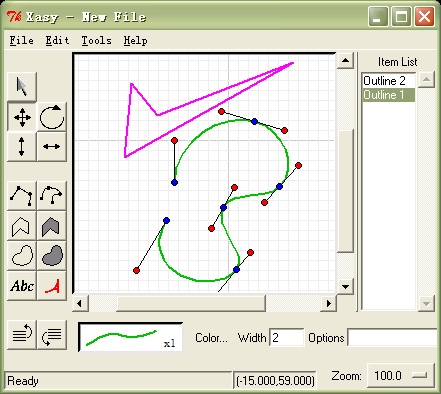
\includegraphics{xasy.png}
  \caption{微软 Windows 系统下运行的 \prgname{Xasy} 界面示例}
  \label{fig:xasy}
\end{figure}

    请运行并熟悉 \prgname{Xasy} 的用法,查看用它生成的代码,并尝试与自己写的
    代码结合起来。
    
    (注:\prgname{Xasy} 会随 \Asy{} 安装在系统中。但在 Windows 下运行
    \prgname{Xasy} 需要自己下载安装 Python $2.6$ 系统及 Python Imaging
    Library,请参考 \cite{asyman} 中的说明。)

  \item 试画出下面的图形(提示:可以把叶子在一个自定义图中画好,在循环中变换
    后用 |add| 加入当前图):
\begin{figure}[H]
  \centering
\begin{asy}
size(8cm,0);
guide leaf_above = (-0.5,0) {dir(30)} .. {dir(-30)} (0.5,0);
guide leaf_below = (-0.5,0) {dir(-30)} .. {dir(30)} (0.5,0);
guide leaf = leaf_above & reverse(leaf_below) & cycle;
picture pic;
fill(pic, leaf, heavygreen);
draw(pic, leaf_above, darkgreen+2);
draw(pic, leaf_below, lightgreen+2);
for (int i = 0; i < 10; ++i)
    for (int j = 0; j < 5; ++j)
        add( shift(i*1.1,j*1.1) * rotate((i+j)*18) * pic );
shipout(bbox(Fill(darkblue)));
\end{asy}
\end{figure}

  \item\label{ex:venn} 利用图形剪裁,绘制两个集合交集 $A \cap B$ 的 Venn 图:
\begin{figure}[H]
  \centering
\begin{asy}
size(0,4cm);
guide a = circle((0,0), 1);
guide b = circle((1,0), 1);
picture inter;
fill(inter, a, lightblue);
clip(inter, b);
add(inter);
label("$A\cap B$", (1/2,0));
draw(a ^^ b, linewidth(0.6));
label(Label("$A$",position=3), a);  // position=3 是圆下方 3 号结点
label(Label("$B$",position=3), b);
\end{asy}
\end{figure}

  \item 与 |clip| 命令作用类似,还有一个
    |unfill|\index{unfill@\asyinline=unfill=} 命令也可以用于图形的剪裁。它们
    的区别是,|clip| 命令留下剪裁曲线的内部,而 |unfill| 命令挖掉剪裁曲线的内
    部而留下外部。|unfill| 命令的语法与 |clip| 相同。借用
    \autoref{sec:clippicture} 中的 |mypic| 举例:
\begin{asycode}
add(mypic);
draw(circle((2cm,2cm), 1.5cm), red+1bp);
unfill(mypic, circle((2cm,2cm), 1.5cm));
add(mypic, (5cm,0));
\end{asycode}
\begin{figure}[H]
  \centering
\begin{asy}
picture mypic;
draw(mypic, (0,0) -- (3cm,4cm) -- (5cm,0) -- cycle, gray+2mm);
fill(mypic, circle((3cm,2cm), 1cm), lightblue);
label(mypic, "triangle", (1cm,0), N);
label(mypic, "circle", (3cm,2cm));
add(mypic);
draw(circle((2cm,2cm), 1.5cm), red+1bp);
unfill(mypic, circle((2cm,2cm), 1.5cm));
add(mypic, (5cm,0));
\end{asy}
\end{figure}

    下面,请利用 |unfill| 命令绘制两个集合差集 $A\setminus B$ 和对称差集
    $A\bigtriangleup B$ 的 Venn 图\footnote{Venn 图的做法并不是唯一的。例如,
    对称差集 $A\bigtriangleup B$ 的 Venn 图也可以利用 \autoref{sec:curve} 绘
    制圆环的方式制做;在 \cite{asyman} 中,还介绍了利用表示特殊填充规则的画笔
    \asyinline=evenodd=\index{evenodd@\asyinline=evenodd=} 绘制这种 Venn 图的
    方法;路径的 \asyinline=buildcycle=
    \index{buildcycle@\asyinline=buildcycle=}函数(参看 \cite{asyman})也可以
    用于绘制对称差集——这些方式对画一般的 Venn 图并不通用,但在一些情况下比
    使用剪裁功能要简洁,或能得到更丰富的效果。读者在实际使用中不必拘泥。}:
\begin{figure}[H]
  \centering
\begin{asy}
size(0,4cm);
guide a = circle((0,0), 1);
guide b = circle((1,0), 1);
picture pic1, pic2;
picture a_minus;
fill(a_minus, a, lightblue);
unfill(a_minus, b);
add(pic1, a_minus);
label(pic1, "$A\setminus B$", (-1/2,0));
draw(pic1, a ^^ b, linewidth(0.6));
label(pic1, Label("$A$",position=3), a);
label(pic1, Label("$B$",position=3), b);
picture b_minus;
fill(b_minus, b, lightblue);
unfill(b_minus, a);
add(pic2, a_minus);
add(pic2, b_minus);
label(pic2, "$A\bigtriangleup B$", (1/2,1.2), N);
draw(pic2, (1/2,1.2)--(0,3/4) ^^ (1/2,1.2)--(1,3/4));
draw(pic2, a ^^ b, linewidth(0.6));
label(pic2, Label("$A$",position=3), a);
label(pic2, Label("$B$",position=3), b);
add(pic1);
add(shift(4)*pic2);
\end{asy}
\end{figure}

  \item 请制做下面的艺术字效果:
\begin{figure}[H]
  \centering
\begin{asy}
settings.tex="xelatex";
usepackage("xeCJK");
texpreamble("\setCJKmainfont{FZHei_GB18030-B01}");
picture hei, bai;
label(hei, "黑白", black+fontsize(4cm));
label(bai, "黑白", white+fontsize(4cm));
fill(hei, box((-5cm,-3cm), (5cm,3cm)), white);
fill(bai, box((-5cm,-3cm), (5cm,3cm)), black);
guide g = (-5cm,-3cm) {right} .. (0,0){down} .. {right} (5cm,3cm);
clip(hei, g -- (-5cm,3cm) -- cycle);
clip(bai, g -- (5cm,-3cm) -- cycle);
add(hei);
add(bai);
\end{asy}
\end{figure}
\end{enumerate}

本章的素材源自 \prgname{PSTricks} 的文档 \cite{pstricks} 中的一个例子。
\prgname{PSTricks} 是 \TeX{} 的一个老牌绘图宏包,功能强大,尤其是与 \LaTeX{} 
文档有很好的结合性。在 \cite{pstricks} 中还可以找到其他一些有趣的铺砌图形。

\Asy{} 的曲线控制方式脱胎于它的前身 \MP{},而 \MP{} 的语法和曲线控制方式则与
其前身 \MF{} 完全相同。\MF{} 是 Knuth 为配合 \TeX{} 系统制做的字体设计软件,
在 \MF{} 的经典文献 \cite{knuth1986} 中详细介绍了这种曲线的控制。\MP{} 是
John D. Hobby 模仿 \MF{} 编写的绘图软件,它与 \Asy{} 采用基本相同的方式使用
\TeX{} 排版文字,\MP{} 的文档 \cite{mpman} 也对曲线控制有一些说明。而介绍与
\mbox{Con\TeX{}t} 配合使用 \MP{} 的著名文档 \emph{METAFUN}\cite{metafun} 更是
以极其详实的例子展示了曲线绘制的各个方面。除个别连接符不同,\Asy{} 的曲线控制
语法与 \MF{} 及 \MP{} 基本相同,本章关于曲线控制的内容也主要参考了这些文档
\cite{knuth1986, mpman, metafun}。

与在 \MF{} 及 \MP{} 不同的是,在 \Asy{} 中,曲线(包括直线)被分为两种不同的
数据类型:|path|(译为路径)和 |guide|(暂译为路向)。在 \MF{} 和 \MP{} 中的
路径(|path| 类型)实际对应于 \Asy{} 中的 |guide|。在计算机中曲线的数学表示是
由一列结点和控制点决定的三次 Bézier 样条曲线,这种确定的曲线在 \Asy{} 中对应
于 |path| 类型;而由 |--|、|..| 等连接符说明的曲线,仍可能在延长时改变形状,
在以一定算法转换为三次 Bézier 样条之前,就是 \Asy{} 中的 |guide| 类型。本章
的内容集中在使用更直观的曲线连接符生成 |guide| 类型的曲线,而完全用数学方式操
控 |path| 类型,将在 \autoref{sec:guide2path} 中进一步介绍。

变量定义、循环和判断是使用 \Asy{} 编程的基础。\Asy{} 的程序设计语法基本来自
C++ 语言,而略有扩充和改动。本教程有意淡化编程语法,也不假定读者有很好的编程
基础,但熟悉 C/C++/Java 语言的读者学习 \Asy{} 会方便得多。如果对 \Asy{} 语言
有疑问,请参考 \Asy{} 的官方手册 \cite{asyman} 或中文的节译。

图类型(|picture|)也源自 \MP{},它是分组绘图和图形复用的基础。不过 \Asy{} 的
图类型功能更复杂,使用 |size| 函数自动缩放就是 \Asy{} 的特色功能。

剪裁功能可以产生许多特殊效果,本章正文只是最简单的应用,习题中展示了剪裁功能
的一些更实际的应用,但仍然有一些问题没有涉及,留待读者自行思考了。

\endinput

% vim:tw=77:

